\documentclass[11pt]{article}
\usepackage[margin=1in]{geometry}
\usepackage{booktabs,graphicx,caption,hyperref,xcolor,enumitem,amsmath}
\hypersetup{colorlinks=true,linkcolor=black,urlcolor=blue!50!black}
\graphicspath{{../results/}{../results/dataset/}{../../results/}{../../slides/assets/}}
\setlist{itemsep=2pt}
\captionsetup{font=small}

\title{Teaching a Small Neural Network to Listen\\\large From counting voices in a noisy room to naming the genre of a song}
\author{Karol D\k{a}browski \\ First-Year Seminar}
\date{28 October 2026}

\begin{document}
\maketitle

\begin{abstract}
This project went through two phases. First I built a small convolutional neural network (CNN) that listens to four seconds of audio and counts how many people are talking. It reached \textbf{80\,\%} exact accuracy on synthetic clips, collapsed to 25\,\% on real meeting recordings, and recovered to 68\,\% after retraining on real data. Then I pivoted to music: the same kind of network, trained on 30-second previews scraped from the Deezer API, names the genre of a song out of eight (classical, pop, jazz, hip-hop, rock, electronic, country, film score). The best from-scratch CNN gets \textbf{77\,\%} on songs by artists it never heard. A tiny classifier placed on top of a large public audio model (CLAP) gets \textbf{79\,\%}, and the two combined \textbf{80\,\%}. Chance is 12.5\,\%. Along the way I built a web demo, tested the models on 500 brand-new songs, and measured how much extra data actually helps.
\end{abstract}


\section{The common idea: sound as a picture}
Every model in this project works the same way. Audio is turned into a \emph{spectrogram}: a picture with time running left to right, pitch running bottom to top, and brightness showing how much energy there is at that pitch and moment. A voice shows up as a stack of horizontal lines (its harmonics). A drum hit is a vertical stripe. A CNN, the kind of network used for images, then reads that picture.

I used the \emph{mel} spectrogram, which spaces the pitch bands the way human hearing does: fine at low pitch, coarse at high pitch. Formally, with $S[k,t]$ the short-time Fourier power and $F$ the mel filterbank,
\[
M[m,t] = \log\Big(\sum_k F_{m,k}\,S[k,t] + 10^{-6}\Big).
\]
Speech clips used 64 bands over 4 seconds; music clips used 128 bands over 30 seconds.

\begin{figure}[h]\centering
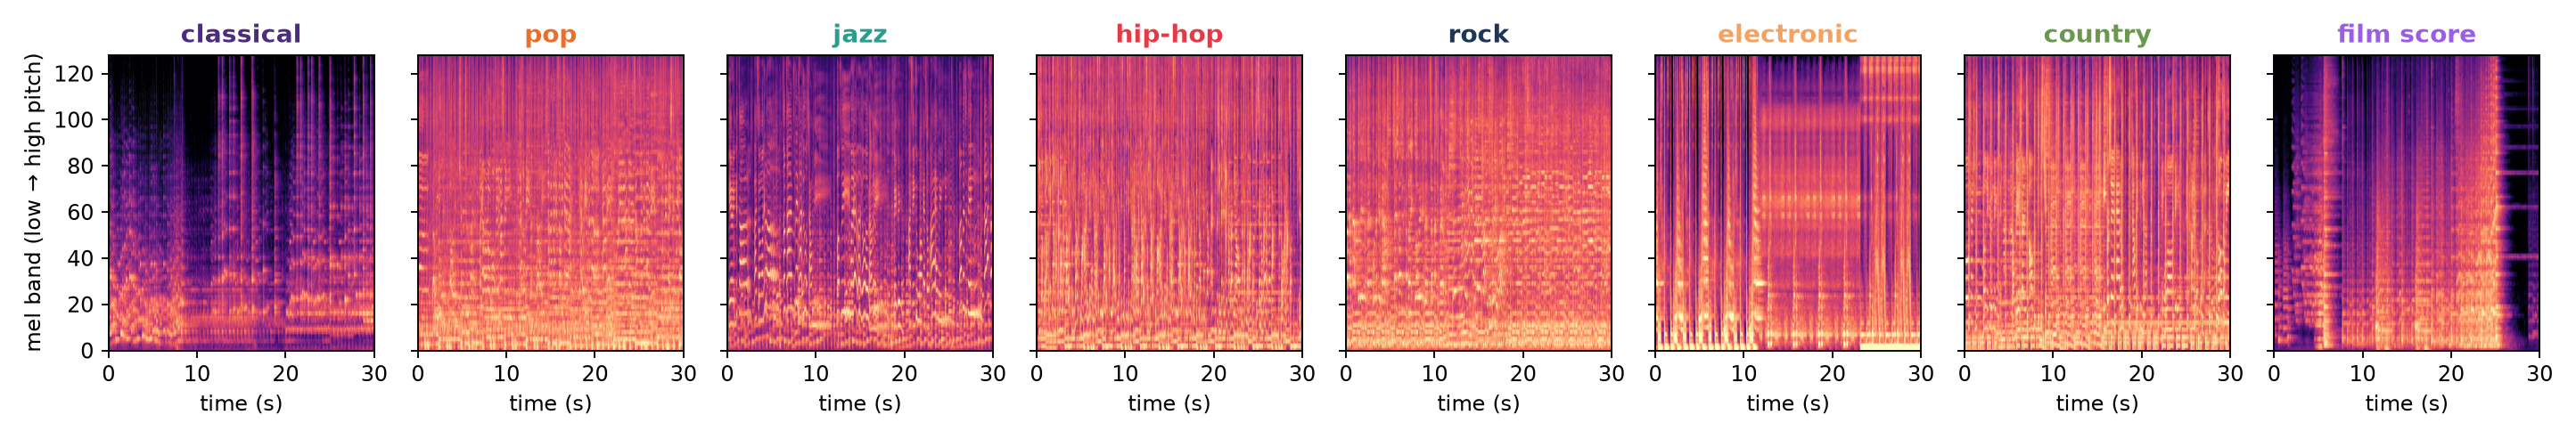
\includegraphics[width=\textwidth]{typical_spectrograms.png}
\caption{One typical 30-second clip per music genre, on the same colour scale. Classical and film score are sparse and quiet, pop, rock and hip-hop are dense walls of sound, electronic has hard-edged blocks and a steady beat.}
\end{figure}

\section{Phase 1: counting voices in a noisy room}

\subsection{Data: a public speech corpus turned into 20\,000 noisy clips}
There is no public dataset of ``$n$ people talking at once'' with exact labels, so I made one.
\begin{itemize}
  \item Source: LibriSpeech, free audiobook readings. 291 speakers (146 male, 145 female), each recorded alone in a quiet room.
  \item Recipe: pick 0 to 4 speakers, overlay a 4-second excerpt from each, add reverb half of the time, add white, pink or ``babble'' noise at 0 to 20\,dB signal-to-noise ratio.
  \item Because I built the clips, the labels (people, male, female) are exact. Test speakers never appear in training.
\end{itemize}

\subsection{Model and results}
A small CNN with four stages of filters (32, 64, 128, 128), a pooled summary of 128 numbers, and three output heads: total people, number of male voices, number of female voices. Trained for 30 passes, about 1.5 hours on the laptop GPU.

\begin{table}[h]\centering\small
\begin{tabular}{lccc}\toprule
 & exact count & within one & \\\midrule
total speakers & 80\,\% & 99\,\% & \\
male voices & 75\,\% & 99\,\% & \\
female voices & 78\,\% & 99\,\% & \\\bottomrule
\end{tabular}
\caption{Best synthetic model (cnn\_v4) on 2\,000 clips from unseen speakers.}
\end{table}
\begin{figure}[h]\centering
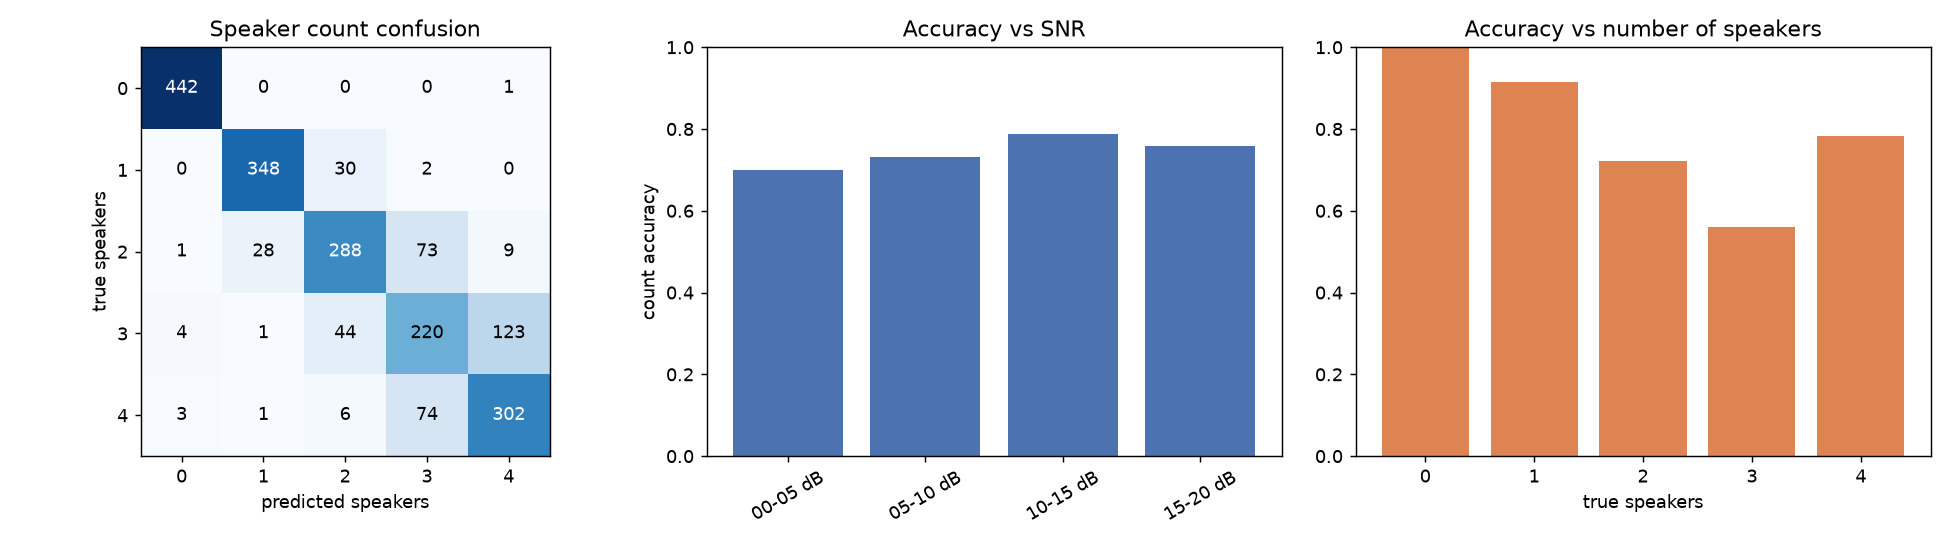
\includegraphics[width=\textwidth]{cnn_v4/summary.png}
\caption{Where the voice counter goes wrong. Three simultaneous speakers is the hard case (56\,\%): three voices are often heard as four, or two. Low signal-to-noise, reverb and babble noise hurt most.}
\end{figure}

\subsection{Experiment: mel spectrogram vs.\ plain spectrogram}
Same clips, same network, same seed, only the input changed. The mel version was 1 to 2 points better (83.4 vs.\ 81.4\,\% on one test set) and trained twice as fast because its input is half the size. One run each, so suggestive rather than proven.

\subsection{Real meetings: the synthetic model collapses, retraining recovers it}
I then tested on the AMI Meeting Corpus, about 100 hours of real four-person meetings recorded with a table microphone, with time-stamped speaker turns that give an exact count for every 4-second window.
\begin{table}[h]\centering\small
\begin{tabular}{lcc}\toprule
model & exact count & within one \\\midrule
cnn\_v4, synthetic only & 25\,\% & 78\,\% \\
cnn\_v6, retrained from scratch on 42\,000 real windows & \textbf{68\,\%} & 97\,\% \\
cnn\_v7, fine-tuned from cnn\_v4 & 66\,\% & 97\,\% \\
always guess ``one speaker'' & 60\,\% & -- \\\bottomrule
\end{tabular}
\caption{8\,000 real test windows from meetings not used in training.}
\end{table}
The synthetic model fails because far-field room audio is quieter and more echoey than anything it saw: it labels most real speech as silence. Retraining fixes that, but two overlapping speakers remain hard (45\,\%), because real overlaps are brief and usually heard as one person. The fine-tuned model also forgot the synthetic task, dropping to 38\,\% there. This was the first big lesson of the project: \emph{a model is only as general as its training data}.

\subsection{Experiment: is counting easier if all voices are the same sex?}
Two new synthetic sets, one all-male, one all-female, same recipe. Specialist models beat the mixed model on their own sex by about 2 points (male 82.2 vs.\ 79.8\,\%, female 78.7 vs.\ 76.5\,\%) but lose 5 to 9 points on the other sex. A real but small gain, so one mixed model is the safer choice. Female voices were harder for every model.
\begin{figure}[h]\centering
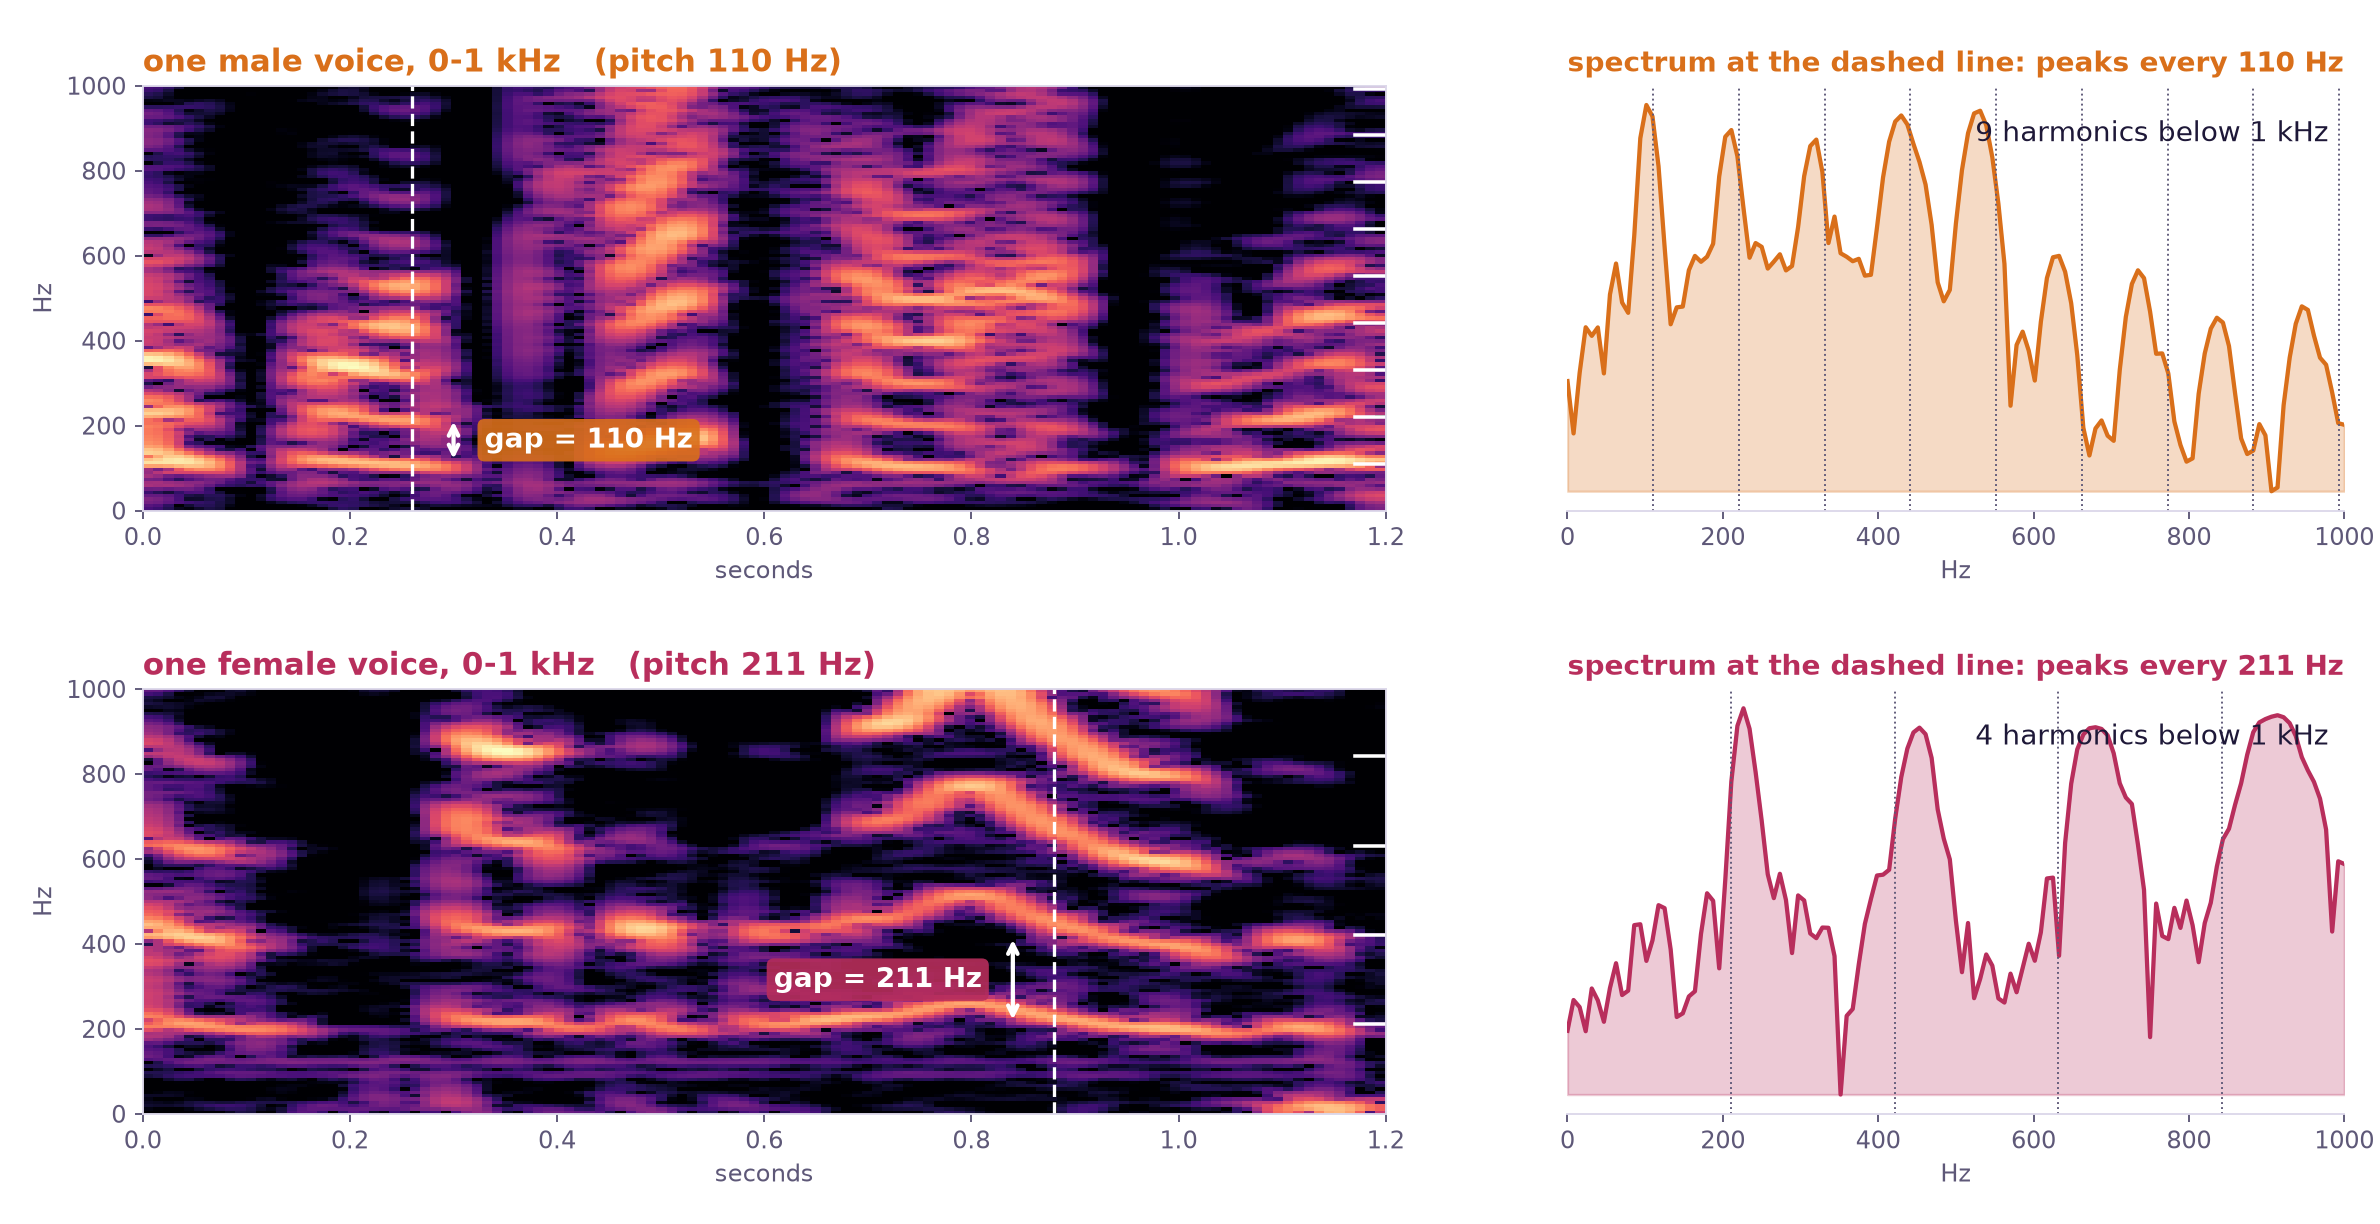
\includegraphics[width=.8\textwidth]{male_vs_female_light.png}
\caption{Why sex matters: one male voice (pitch 110\,Hz) and one female voice (211\,Hz). Female harmonics are spaced about twice as far apart, and two or three overlapping female voices blur together more easily.}
\end{figure}

\subsection{A human check}
I took the test myself on 40 clips: 45\,\% exact against the model's 75\,\% on the same clips. Counting overlapping voices is hard for people too.

\section{Phase 2: the pivot to music genre}

\subsection{Why}
Speaker counting had reached a plateau set by the data, and the same tools apply directly to music: a spectrogram in, a label out. The question changed from ``how many?'' to ``what kind?'', with seven broad genres at first and film score added later.

\subsection{Data: scraping Deezer}
Spotify no longer gives out audio previews, so I used Deezer's public API, which serves a 30-second MP3 for almost any track with no key.
\begin{itemize}
  \item For each genre, start from Deezer's genre charts, playlists and radios, then walk to related artists.
  \item Keep an artist only if at least half of their albums carry that genre tag. The label of a track is its album's genre tag.
  \item At most 12 tracks per artist and 4 per album, so no single artist dominates. An artist can only be in one genre.
  \item Film score: Deezer's ``Films/Games'' tag is full of pop songs from movies, so I seeded from 65 film and game composers instead and skipped the charts.
  \item Split by \emph{artist}, 80/10/10. Every test song is by an artist the model never heard. This matters: splitting by song would let the model recognise artists instead of genres.
\end{itemize}
First crawl: 12\,699 clips from about 1\,100 artists. A second crawl later doubled this to 25\,943 clips, adding only new artists and leaving the validation and test clips untouched. Two practical lessons: preview links expire within minutes, so download immediately; and after about 10\,000 fast downloads the server starts refusing, so go slowly.

\begin{figure}[h]\centering
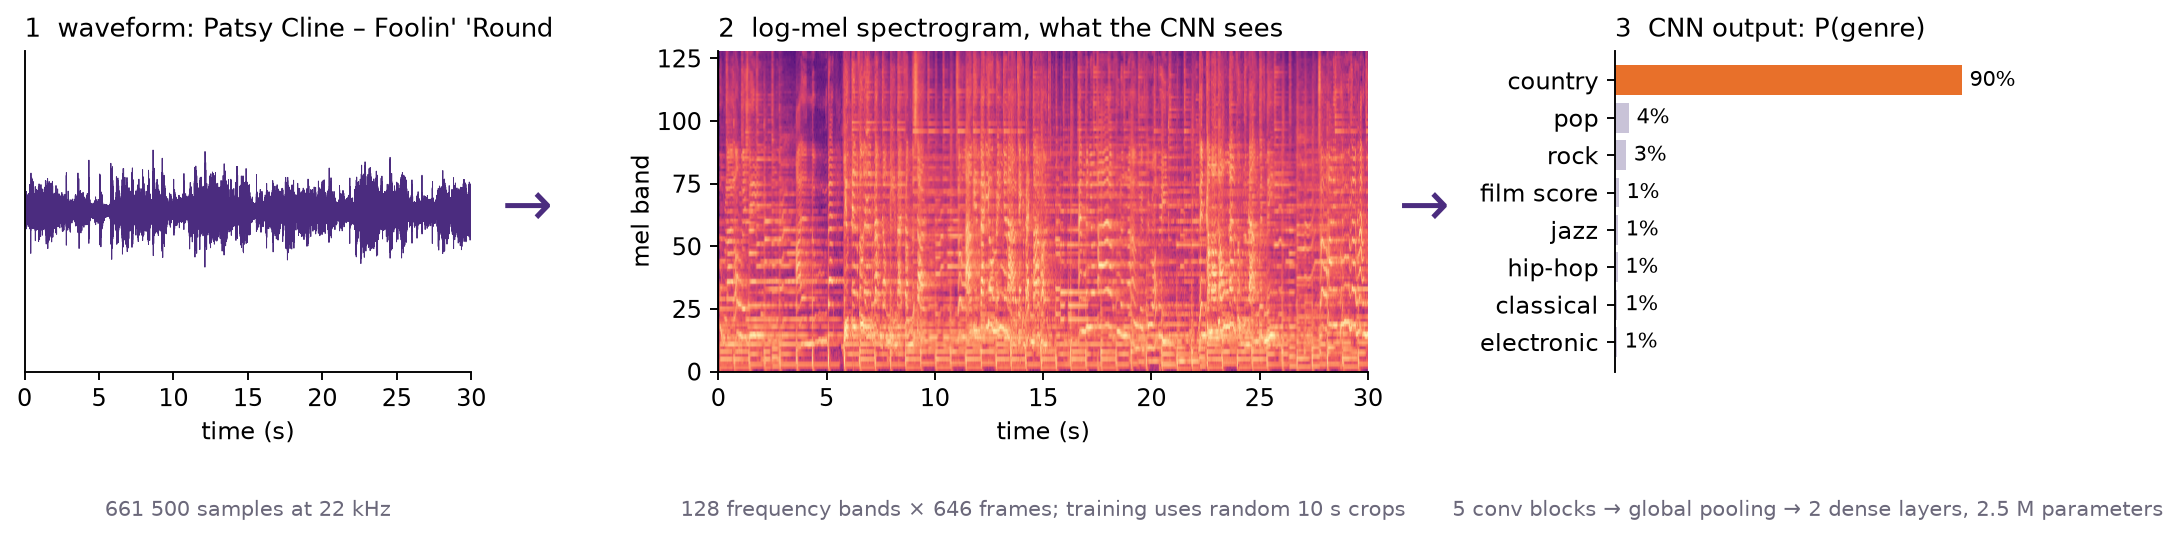
\includegraphics[width=\textwidth]{pipeline_example.png}
\caption{One test clip through the pipeline: waveform, log-mel spectrogram, and the network's output.}
\end{figure}

\subsection{Model}
The same family of CNN as before, slightly bigger: five stages of filters, global pooling, two dense layers, 2.5 million parameters (later 5.5 million). Training looks at random 10-second crops with parts of the spectrogram masked out (``SpecAugment''), which acts like showing the network many more clips than it has. Testing uses the full 30 seconds.

\subsection{Results of the from-scratch CNN}
\begin{table}[h]\centering\small
\begin{tabular}{lcccc}\toprule
model & genres & training clips & test accuracy & macro F1 \\\midrule
cnn\_v2 & 7 & 9\,000 & 79.2\,\% & 0.79 \\
cnn\_v3 (adds film score, fine-tuned from cnn\_v2) & 8 & 10\,200 & 75.4\,\% & 0.75 \\
cnn\_v4 (bigger, trained from scratch) & 8 & 23\,500 & \textbf{77.4\,\%} & 0.77 \\\bottomrule
\end{tabular}
\caption{Genre CNNs on the test split (1\,204 clips for 8 genres). Chance is 12.5\,\%. Macro F1 is the average of per-genre F1 scores, so every genre counts equally.}
\end{table}
\begin{figure}[h]\centering
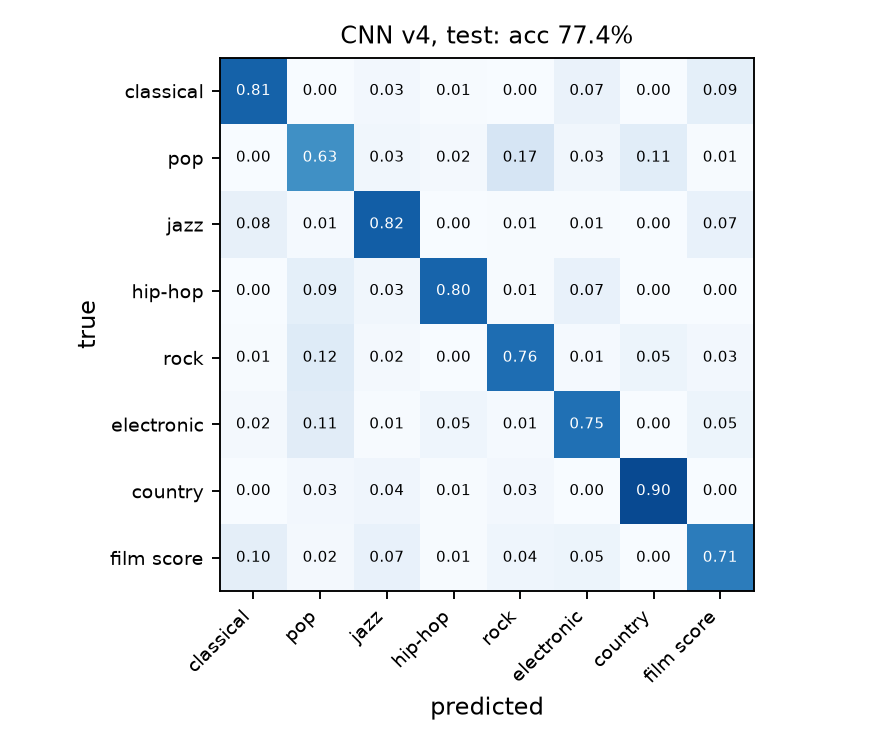
\includegraphics[width=.49\textwidth]{confusion_cnn_v4_w48_test.png}\hfill
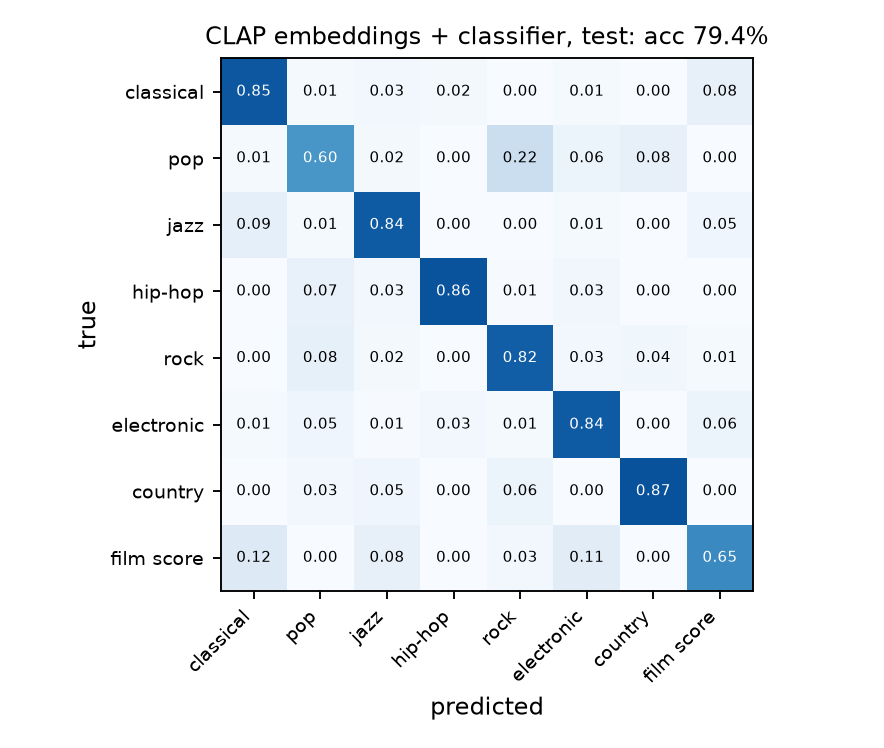
\includegraphics[width=.49\textwidth]{confusion_clap_head_test.png}
\caption{Confusion matrices on the test split: rows are the true genre, columns the prediction, each row sums to one. Left: the CNN. Right: the CLAP-based classifier from Section~\ref{sec:clap}.}
\end{figure}
Two patterns dominate the errors, and they never went away in any model:
\begin{itemize}
  \item \textbf{Pop is a catch-all.} Around a quarter of pop songs are called rock or country, and every other genre leaks about 10\,\% into pop. This is a label problem, not a model problem: Deezer tags whole albums, and ``pop'' means many things.
  \item \textbf{Classical and film score sound alike.} Adding film score cost classical recall, from 90\,\% to 67\,\%. One in five classical clips is now called a score. Same orchestra, different production.
\end{itemize}
More audio helps: with only 2 seconds of a song the CNN gets 52\,\%, with 5 seconds 67\,\%, with 10 seconds 75\,\%, and with 30 seconds 76\,\%.

\subsection{A live demo}
A small local web page (\texttt{src/app.py}): drop any MP3 of any length, or type a song name, and it shows the album cover, a 10-second player, the probability for every genre, and the spectrogram with the network's guess written over each 5-second window. It can also run several models side by side. In class examples: Beethoven $\to$ classical 94\,\%, Miles Davis $\to$ jazz 97\,\%, Kendrick Lamar $\to$ hip-hop 97\,\%, Hans Zimmer's ``Time'' $\to$ film score 90\,\%, and Dolly Parton's ``Jolene'' split 49\,\% country / 46\,\% pop.

\section{Phase 3: comparing against a large public model}\label{sec:clap}

\subsection{What CLAP is}
CLAP (Contrastive Language-Audio Pretraining, from LAION) is a model trained on hundreds of thousands of audio clips paired with text captions. It turns any clip into a list of 512 numbers (an \emph{embedding}) and any sentence into another list of 512 numbers, arranged so that matching sound and text land close together. It has heard far more music than my crawl could collect. I used it in two ways.

\textbf{Zero-shot.} No training at all. Embed the clip, embed eight sentences such as ``this is country music'', and pick the closest. The probability for genre $c$ is
\[
p_c = \operatorname{softmax}_c\big(\tau\cos(\mathbf{a},\mathbf{t}_c)\big),
\]
with $\mathbf{a}$ the audio embedding, $\mathbf{t}_c$ the averaged text embedding for genre $c$, and $\tau\approx39$ a scale CLAP learned. Change the sentences and you change the classifier.

\textbf{Embeddings plus a small classifier.} Embed each of my clips once, then train a tiny network (512 inputs, 256 hidden, 8 outputs, 130\,000 parameters) on those numbers with my labels. CLAP itself is frozen. Training took three minutes.

\subsection{A fresh test set}
To make sure no number was a lucky split, I scraped 504 more clips, 63 per genre, from 258 artists that appear nowhere in the training, validation or test data, and scored every model on them as well.

\subsection{The final comparison}
\begin{table}[h]\centering\small
\begin{tabular}{lrcccc}\toprule
 & trained params & test acc & test F1 & fresh acc & fresh F1 \\\midrule
cnn\_v3 (2.5\,M, 10k clips) & 2.5\,M & 75.4\,\% & 0.75 & 77.8\,\% & 0.78 \\
cnn\_v4 (5.5\,M, 23k clips) & 5.5\,M & 77.4\,\% & 0.77 & 79.4\,\% & 0.79 \\
CLAP zero-shot & 0 & 69.4\,\% & 0.70 & 72.8\,\% & 0.73 \\
CLAP embeddings $+$ small classifier & 0.13\,M & 79.4\,\% & 0.79 & 81.3\,\% & 0.81 \\
ensemble: cnn\_v4 $+$ CLAP classifier & -- & \textbf{79.7\,\%} & \textbf{0.80} & \textbf{81.5\,\%} & \textbf{0.81} \\\bottomrule
\end{tabular}
\caption{All genre models on the frozen test split (1\,204 clips) and the fresh set (504 clips, 258 new artists). Chance is 12.5\,\%.}
\end{table}
\begin{table}[h]\centering\small
\begin{tabular}{lcc|cc}\toprule
 & \multicolumn{2}{c|}{test F1} & \multicolumn{2}{c}{fresh F1} \\
genre & cnn\_v4 & CLAP classifier & cnn\_v4 & CLAP classifier \\\midrule
classical & 0.81 & 0.82 & 0.86 & 0.82 \\
pop & 0.62 & 0.65 & 0.59 & 0.69 \\
jazz & 0.80 & 0.81 & 0.84 & 0.83 \\
hip-hop & 0.85 & 0.91 & 0.93 & 0.95 \\
rock & 0.76 & 0.77 & 0.81 & 0.78 \\
electronic & 0.75 & 0.80 & 0.70 & 0.84 \\
country & 0.88 & 0.88 & 0.87 & 0.81 \\
film score & 0.71 & 0.70 & 0.75 & 0.79 \\\bottomrule
\end{tabular}
\caption{Per-genre F1. The CLAP classifier wins on electronic, pop and film score; the CNN holds its own on country and classical.}
\end{table}

What the table says:
\begin{itemize}
  \item \textbf{Zero-shot CLAP is impressive for zero training} but loses to my small CNN. Its biggest error is calling electronic music pop: 40 of the 63 fresh electronic clips. Its answers also depend on how the prompts are worded, which I never tuned.
  \item \textbf{Transfer beats scratch.} 130\,000 trained parameters on top of CLAP's embeddings beat a 5.5-million-parameter CNN trained on twice the data. CLAP already knows what music sounds like; my labels only have to teach it where my genre boundaries are.
  \item \textbf{The ensemble barely helps} ($+0.3$ points), which means the two models fail on the same clips. Those are the genuinely ambiguous ones, pop above all.
  \item \textbf{More data helps, modestly.} Doubling the clips and widening the network bought 2 points. The learning curve suggests 100\,000 clips would land in the low 80s, not 90. Published human agreement on broad genre labels is about 75 to 85\,\%, so the models are near the ceiling the labels allow.
\end{itemize}

\section{What I learned}
\begin{itemize}
  \item \textbf{Data decides.} The voice counter went from 80\,\% to 25\,\% when the room changed. The genre model's errors are mostly in the labels. In both phases the biggest gains came from better data, not a better network.
  \item \textbf{Test on unseen sources.} Splitting by speaker, and later by artist, kept every number honest. The fresh 500-song set confirmed the test split was representative.
  \item \textbf{Start from a pretrained model when one exists.} Three minutes of training on CLAP embeddings beat two hours of training from scratch.
  \item \textbf{Build the demo.} Playing a song and watching the prediction change every 5 seconds taught me more about the model than the confusion matrix did.
  \item \textbf{Practical things that cost hours:} expiring download links, a server that throttles after 10\,000 requests, a public model that silently loads broken under a new library version, and a laptop that throttles its GPU three-fold the moment the charger is unplugged.
\end{itemize}

\section{Next steps}
\begin{itemize}
  \item Tune the CLAP prompts on the validation split, then fine-tune CLAP's audio encoder itself on my data.
  \item Give cnn\_v4 a longer schedule: its validation accuracy was still rising when training stopped.
  \item Clean up pop: drop albums whose tag disagrees with the artist's majority genre, or allow two labels per song.
  \item Scale to 100\,000 clips as an overnight run, with a 10-million-parameter network and a loader that streams features from disk.
\end{itemize}

\section*{Code and files}
Everything lives in \texttt{\textasciitilde/Desktop/College/FYS}. Phase 1 in \texttt{src/} and \texttt{results/}; Phases 2 and 3 in \texttt{genre/src/} (scraping, preprocessing, training, evaluation, CLAP scripts and the demo app), with all numbers in \texttt{genre/results/comparison.json} and the slide decks in \texttt{slides/} and \texttt{genre/slides/}.
\end{document}
